\documentclass[10pt]{article}

\usepackage[margin=0.72in]{geometry}
\usepackage[T1]{fontenc}
\usepackage[utf8]{inputenc}
\usepackage{microtype}
\usepackage{graphicx}
\usepackage{booktabs}
\usepackage{tabularx}
\usepackage{array}
\usepackage{xcolor}
\usepackage{caption}
\usepackage{subcaption}
\usepackage{amsmath}
\usepackage{enumitem}
\usepackage{hyperref}
\usepackage{float}
\usepackage{longtable}

\definecolor{ink}{HTML}{191D22}
\definecolor{muted}{HTML}{5C6470}
\definecolor{accent}{HTML}{B3392C}
\definecolor{soft}{HTML}{F4F0EA}
\definecolor{line}{HTML}{D7D0C7}

\hypersetup{
  colorlinks=true,
  linkcolor=accent,
  urlcolor=accent,
  citecolor=accent,
  pdftitle={Heuristic Learning Control Across FluidGym and Beacon},
  pdfauthor={Codex}
}

\captionsetup{
  labelfont={bf,color=ink},
  font=small,
  textfont={color=muted},
  skip=5pt
}

\setlength{\parindent}{0pt}
\setlength{\parskip}{5pt}
\setlist[itemize]{leftmargin=*, topsep=2pt, itemsep=2pt}
\renewcommand{\arraystretch}{1.18}
\newcolumntype{Y}{>{\raggedright\arraybackslash}X}
\newcolumntype{L}[1]{>{\raggedright\arraybackslash}p{#1}}

\newcommand{\score}[1]{\textbf{#1}}
\newcommand{\code}[1]{\texttt{\small #1}}
\newcommand{\sourcepath}[1]{\caption*{\footnotesize Source: \path{#1}}}
\newcommand{\tightcaption}[1]{\caption{\small #1}}
\newcommand{\callout}[1]{%
  \vspace{0.35em}
  \noindent\fcolorbox{line}{soft}{%
    \begin{minipage}{0.965\linewidth}
    \color{ink}\small #1
    \end{minipage}
  }
  \vspace{0.35em}
}

\begin{document}
\pagenumbering{gobble}

\begin{titlepage}
  \centering
  \vspace*{0.7in}
  {\Huge\bfseries Heuristic Learning Control\par}
  \vspace{0.15in}
  {\Large FluidGym and Beacon cases, compressed into one evidence-first report\par}
  \vspace{0.35in}
  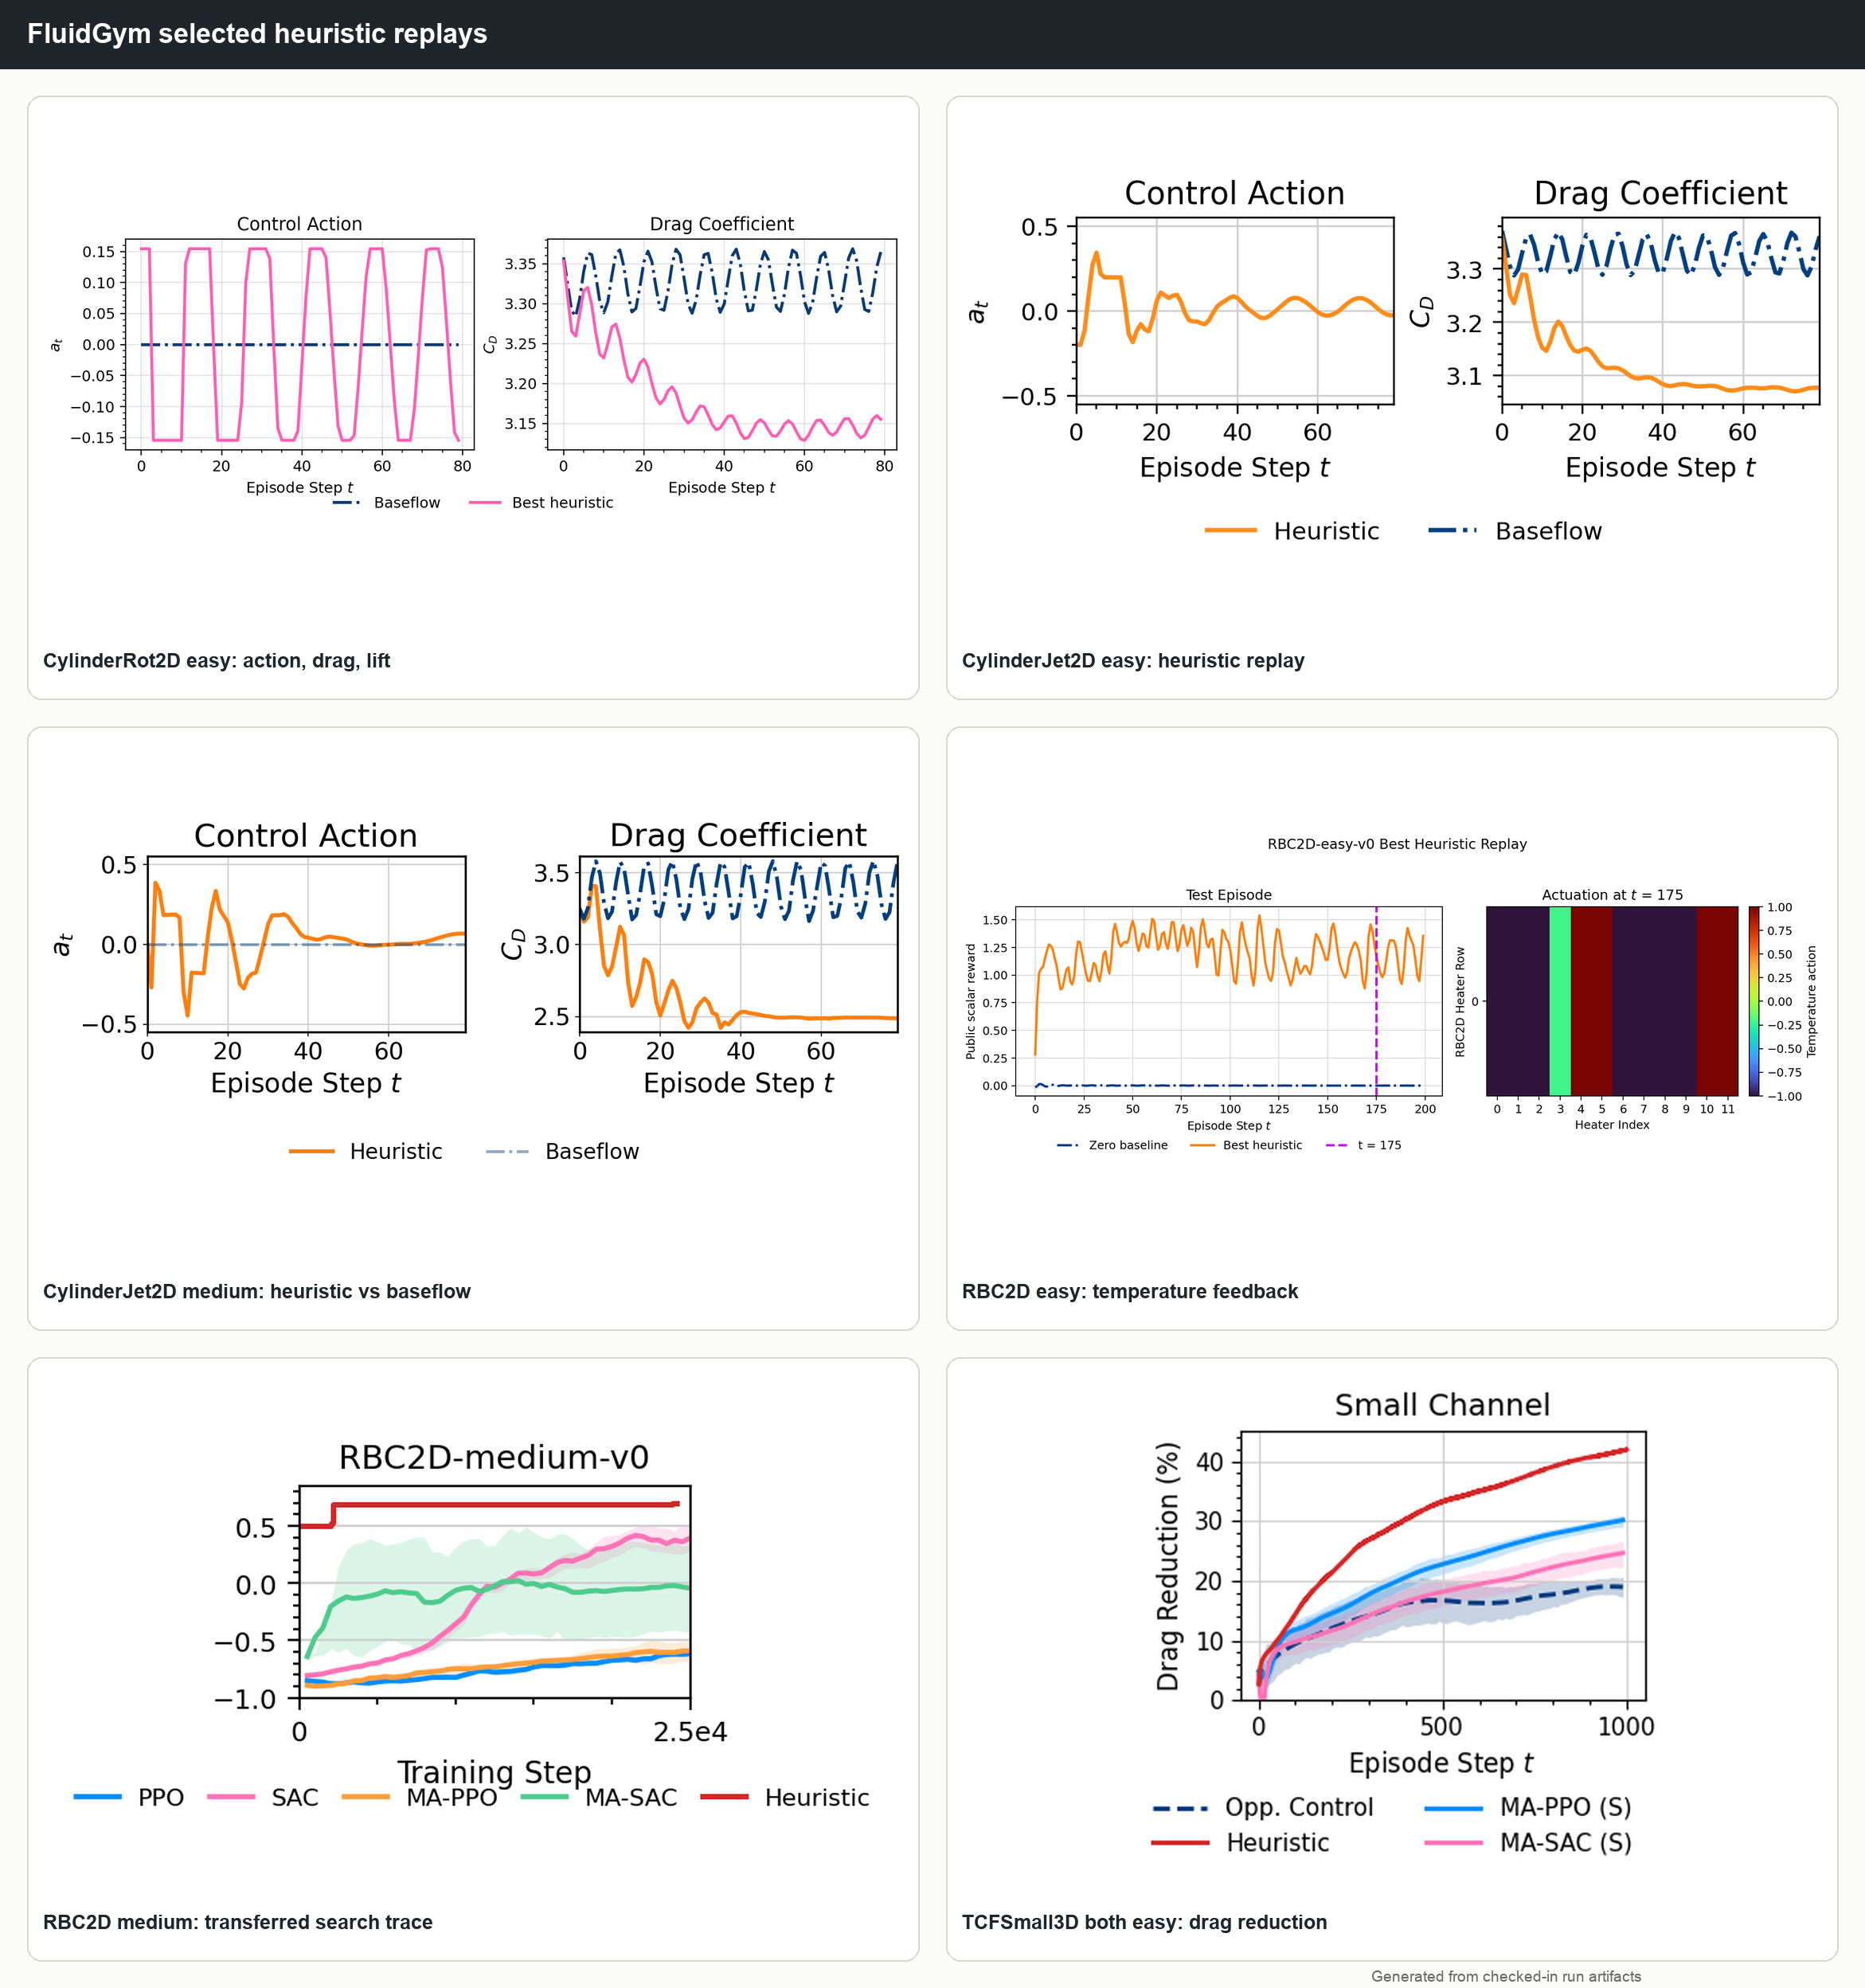
\includegraphics[width=0.88\linewidth]{figures/fluidgym_replay_gallery.png}
  \vfill
  {\large Compiled from local run artifacts in \code{/Users/paulgarnier/github/phd/hl-fluidgym}\par}
  \vspace{0.1in}
  {\large May 15, 2026\par}
\end{titlepage}

\pagenumbering{roman}
\tableofcontents
\clearpage
\pagenumbering{arabic}

\section{Executive Verdict}

The evidence supports a blunt conclusion: the best handcrafted controllers here aren't toys. They are compact, state-aware control laws that reach or beat published learned baselines in several target cases, while costing a tiny fraction of the search budget.

\callout{\textbf{Confidence: high} for metrics copied from JSON, CSV, and markdown artifacts in this workspace. \textbf{Confidence: moderate} for comparisons against paper tables where the objective is aligned but evaluation protocols differ. \textbf{Confidence: low} for any claim about generalization outside these saved seeds and replay protocols.}

The strongest FluidGym wins are \textbf{RBC2D-easy} and \textbf{TCFSmall3D-both-easy}. RBC2D-easy reaches a 5-seed held-out mean step reward of \score{1.1093}, above the paper table's MA-PPO reward of \score{1.024}. TCFSmall3D-both-easy reaches a best mean step reward of \score{0.3068}, above the paper MA-PPO reference of \score{0.207}; the one-episode drag-reduction trace reports \score{30.26\%} mean drag reduction and \score{41.93\%} final drag reduction.

The cylinder cases are strong but uneven. CylinderJet2D-medium finds a \score{0.2433} peak heuristic score and a \score{0.2138} 15-seed expected-score controller, which is basically D-MPC-level on the reported reward but still below SAC's \score{0.426}. CylinderRot2D-easy gets the drag close to SAC, but its held-out reward remains negative.

The Beacon bundle changed materially after the May 15 runs. Lorenz is still the clean scalar hit: \score{477/500} steps in the desired half-space. Vortex now has a valid bounded-action open-loop phase schedule scoring \score{62.4213}, up from the old phase-lock score of \score{23.2389}. Rayleigh's best modal Nusselt-focused heuristic reaches \score{-113.3135}, close to the paper-visual PPO/TD3 reference near \score{-105} but still short of the \score{-100} target. Shkadov is no longer a weak transfer story: the stable delayed shape-feedback law scores \score{50/50} hits on seeds 0--49 and \score{138/138} hits on seeds 0--137, with mean score \score{-0.3443}. Mixing is the bad news: the valid wall-action-only search is still stuck at \score{-7.4252}, while the \score{-1.2969} run edits simulator concentration state and is therefore an invalid boundary probe, not a valid controller.

\section{Evidence Base}

The report uses local artifacts only. No external facts were added. When the report compares a heuristic to PPO, SAC, MA-PPO, MA-SAC, or D-MPC, the comparison comes from the checked-in paper tables under \path{paper/tables}.

\begin{table}[H]
\centering
\small
\begin{tabularx}{\linewidth}{L{0.23\linewidth}Y}
\toprule
Artifact class & Files used \\
\midrule
FluidGym result reports &
\path{cylinder_rot_2d_easy_24h/continuation_report.md},
\path{cylinder_jet_2d_easy/easy_experiment_wrapup.md},
\path{cylinder_jet_2d_medium_24h_improvement/continuation_report.md},
\path{rbc_2d_easy_24h_final/FINAL_WRAPUP.md},
\path{rbc_2d_medium_transfer_50k/transfer_report.md},
\path{tcf_small_3d_both_easy_heuristic_package/run_artifacts/FINAL_REPORT.md}. \\
FluidGym manifests and CSVs &
\path{best_policy_manifest.json}, \path{final_validation_summary.json},
\path{top_policy_summary.csv}, \path{final_best_heuristic_run_summary.json},
\path{heuristic_one_episode_drag_reduction_summary.json}. \\
Beacon replay summaries &
\path{beacon/*/summary.json}, \path{beacon/mixing_target_minus_5/README.md},
\path{beacon/rayleigh_target_minus_100/best_modal_nusselt/manifest.json},
\path{beacon/vortex_target_100_attempt/manifest.json},
\path{beacon/shkadov_stable_search/*summary.json},
\path{beacon/heuristic_strategy_descriptions/strategy_explanations.md}. \\
Paper comparison tables &
\path{paper/tables/Cylinder_results_table.tex},
\path{paper/tables/RBC_results_table.tex},
\path{paper/tables/TCF_results_table.tex}. \\
Figures &
Existing PNG/PDF plots from the result folders, plus contact sheets generated by \path{report/build_galleries.py}. \\
\bottomrule
\end{tabularx}
\caption{Source ledger. The numbers in this report are copied from these artifacts or computed directly from their CSV rows.}
\end{table}

\section{FluidGym Results}

\begin{table}[H]
\centering
\scriptsize
\begin{tabularx}{\linewidth}{L{0.17\linewidth}L{0.16\linewidth}L{0.18\linewidth}L{0.17\linewidth}Y}
\toprule
Case & Selected heuristic & Main score & Comparison anchor & Mechanism \\
\midrule
CylinderRot2D-easy &
\code{pid\_periodic} &
5 held-out mean reward \score{-0.1176}. Seed-0 replay drag \score{3.1821} vs baseflow \score{3.3279}, a \score{4.38\%} drag reduction. &
Paper SAC reward \score{0.037}, drag improvement \score{4.477\%}. &
Capped wall rotation, public lift or antisymmetric sensor proxy, derivative term, tiny sinusoidal carrier. \\
CylinderJet2D-easy &
Full sensor lift-proxy feedback &
5-seed mean reward \score{-0.1255}; replay drag \score{3.1206} vs baseflow \score{3.3281}, a \score{6.24\%} drag reduction. &
Paper SAC reward \score{0.051}, drag improvement \score{6.697\%}. &
302-weight public sensor proxy for lift, one-step derivative damping, single jet action. \\
CylinderJet2D-medium &
PID feedback on lift &
Peak score \score{0.2433}; 15-seed expected-score controller mean \score{0.2138}; replay \score{0.2026} vs baseflow \score{-1.6513}. &
Paper D-MPC reward \score{0.243}; SAC reward \score{0.426}. &
Public lift PID: gain 0.18, derivative 1.60 to 1.625, integral 0.009, integral cap 4. \\
RBC2D-easy &
Spatial temperature feedback &
5 held-out mean reward \score{1.1093}; replay reward \score{1.1935} vs zero baseline \score{0.0001}. &
Paper MA-PPO reward \score{1.024}; MA-SAC \score{0.650}. &
12-heater mean-free local temperature law, square-root contrast, gain 5.0, no smoothing. \\
RBC2D-medium &
Transferred spatial temperature feedback &
Grouped fixed-development score \score{0.6292}; frozen transfer smoke score \score{0.4971}. Held-out rerun skipped. &
Paper SAC reward \score{0.790}; PPO \score{0.138}; MA-PPO \score{0.056}; MA-SAC \score{-0.018}. &
RBC2D-easy law carried to medium with smoothing 0.3. \\
TCFSmall3D-both-easy &
Local mean-free wall feedback &
Best reward \score{0.3068}; fixed replay \score{0.3016}; mean drag reduction \score{30.26\%}. &
Paper MA-PPO reward \score{0.207}; MA-SAC \score{0.171}. &
Translation-equivariant per-wall centering, normalization, one smoothing pass, channel-0 residual, mean-free action. \\
\bottomrule
\end{tabularx}
\caption{FluidGym case results. The table mixes held-out validation, fixed-seed replay, and grouped development selection; the validation basis is stated in each row because smearing those protocols together would be bad accounting.}
\end{table}

\begin{figure}[H]
\centering
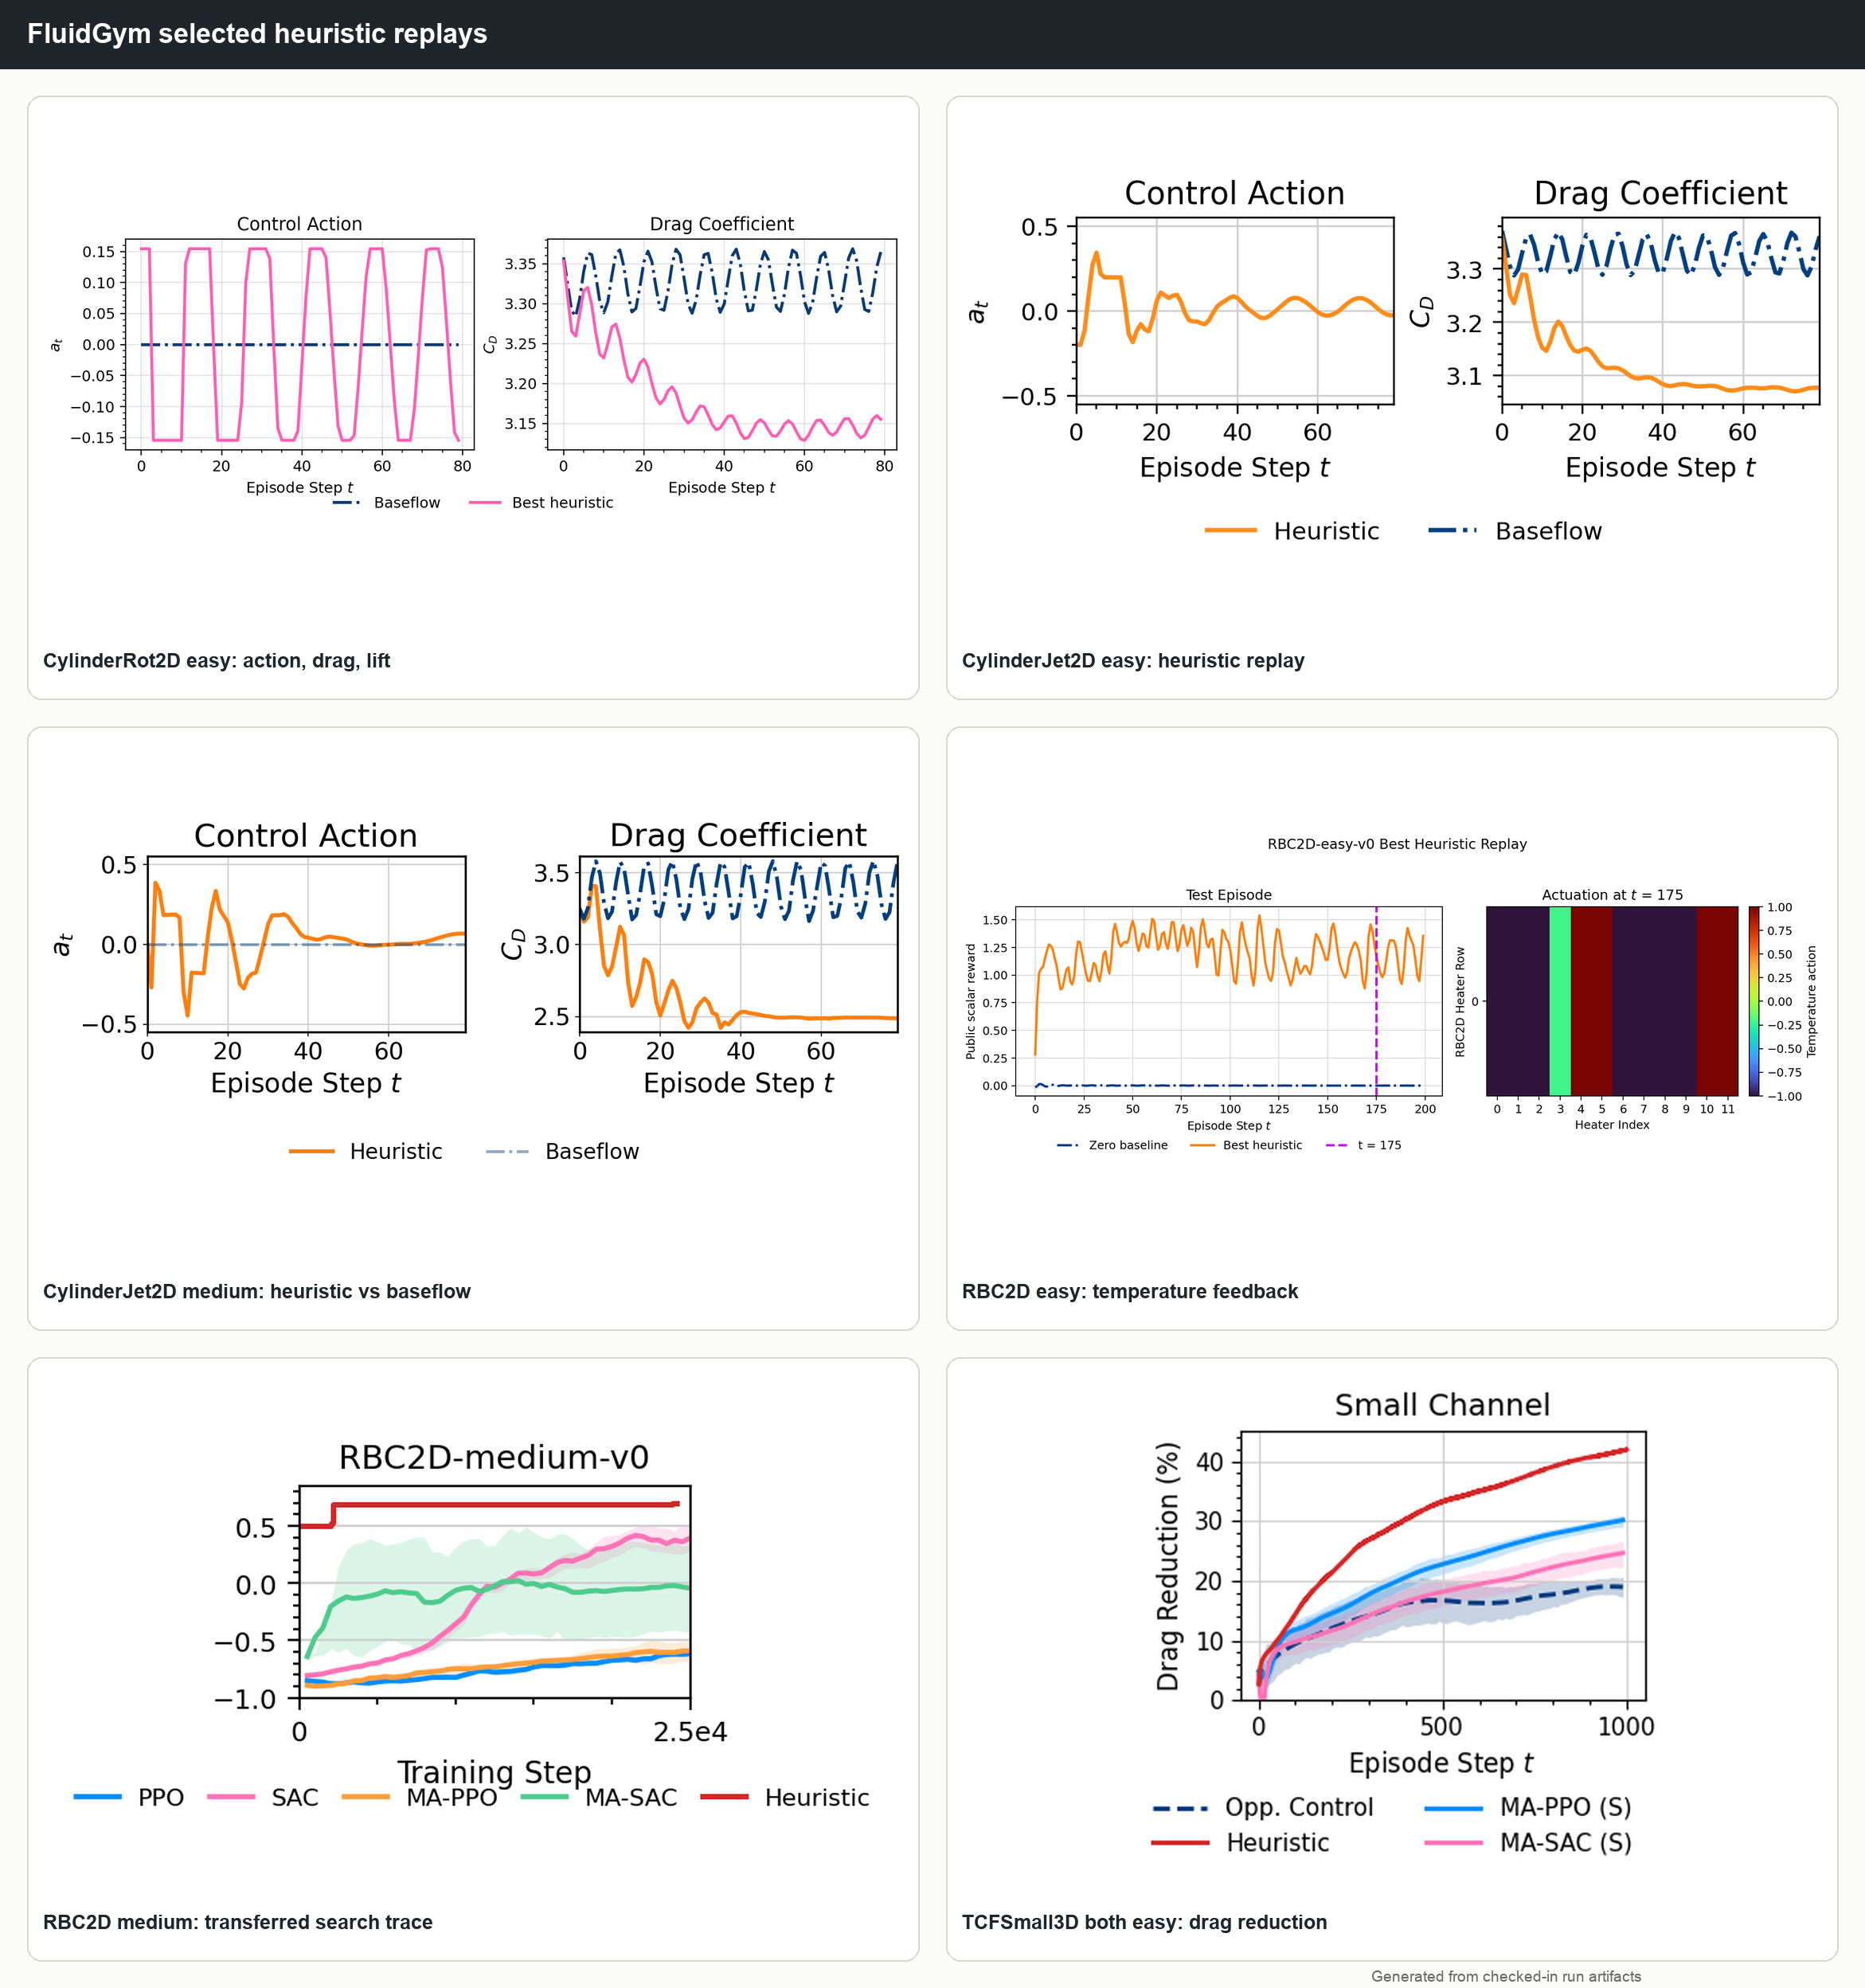
\includegraphics[width=\linewidth]{figures/fluidgym_replay_gallery.png}
\caption{Selected FluidGym replay plots. Each tile comes from the corresponding run artifact folder; the contact sheet only packs them together.}
\end{figure}

\begin{figure}[H]
\centering
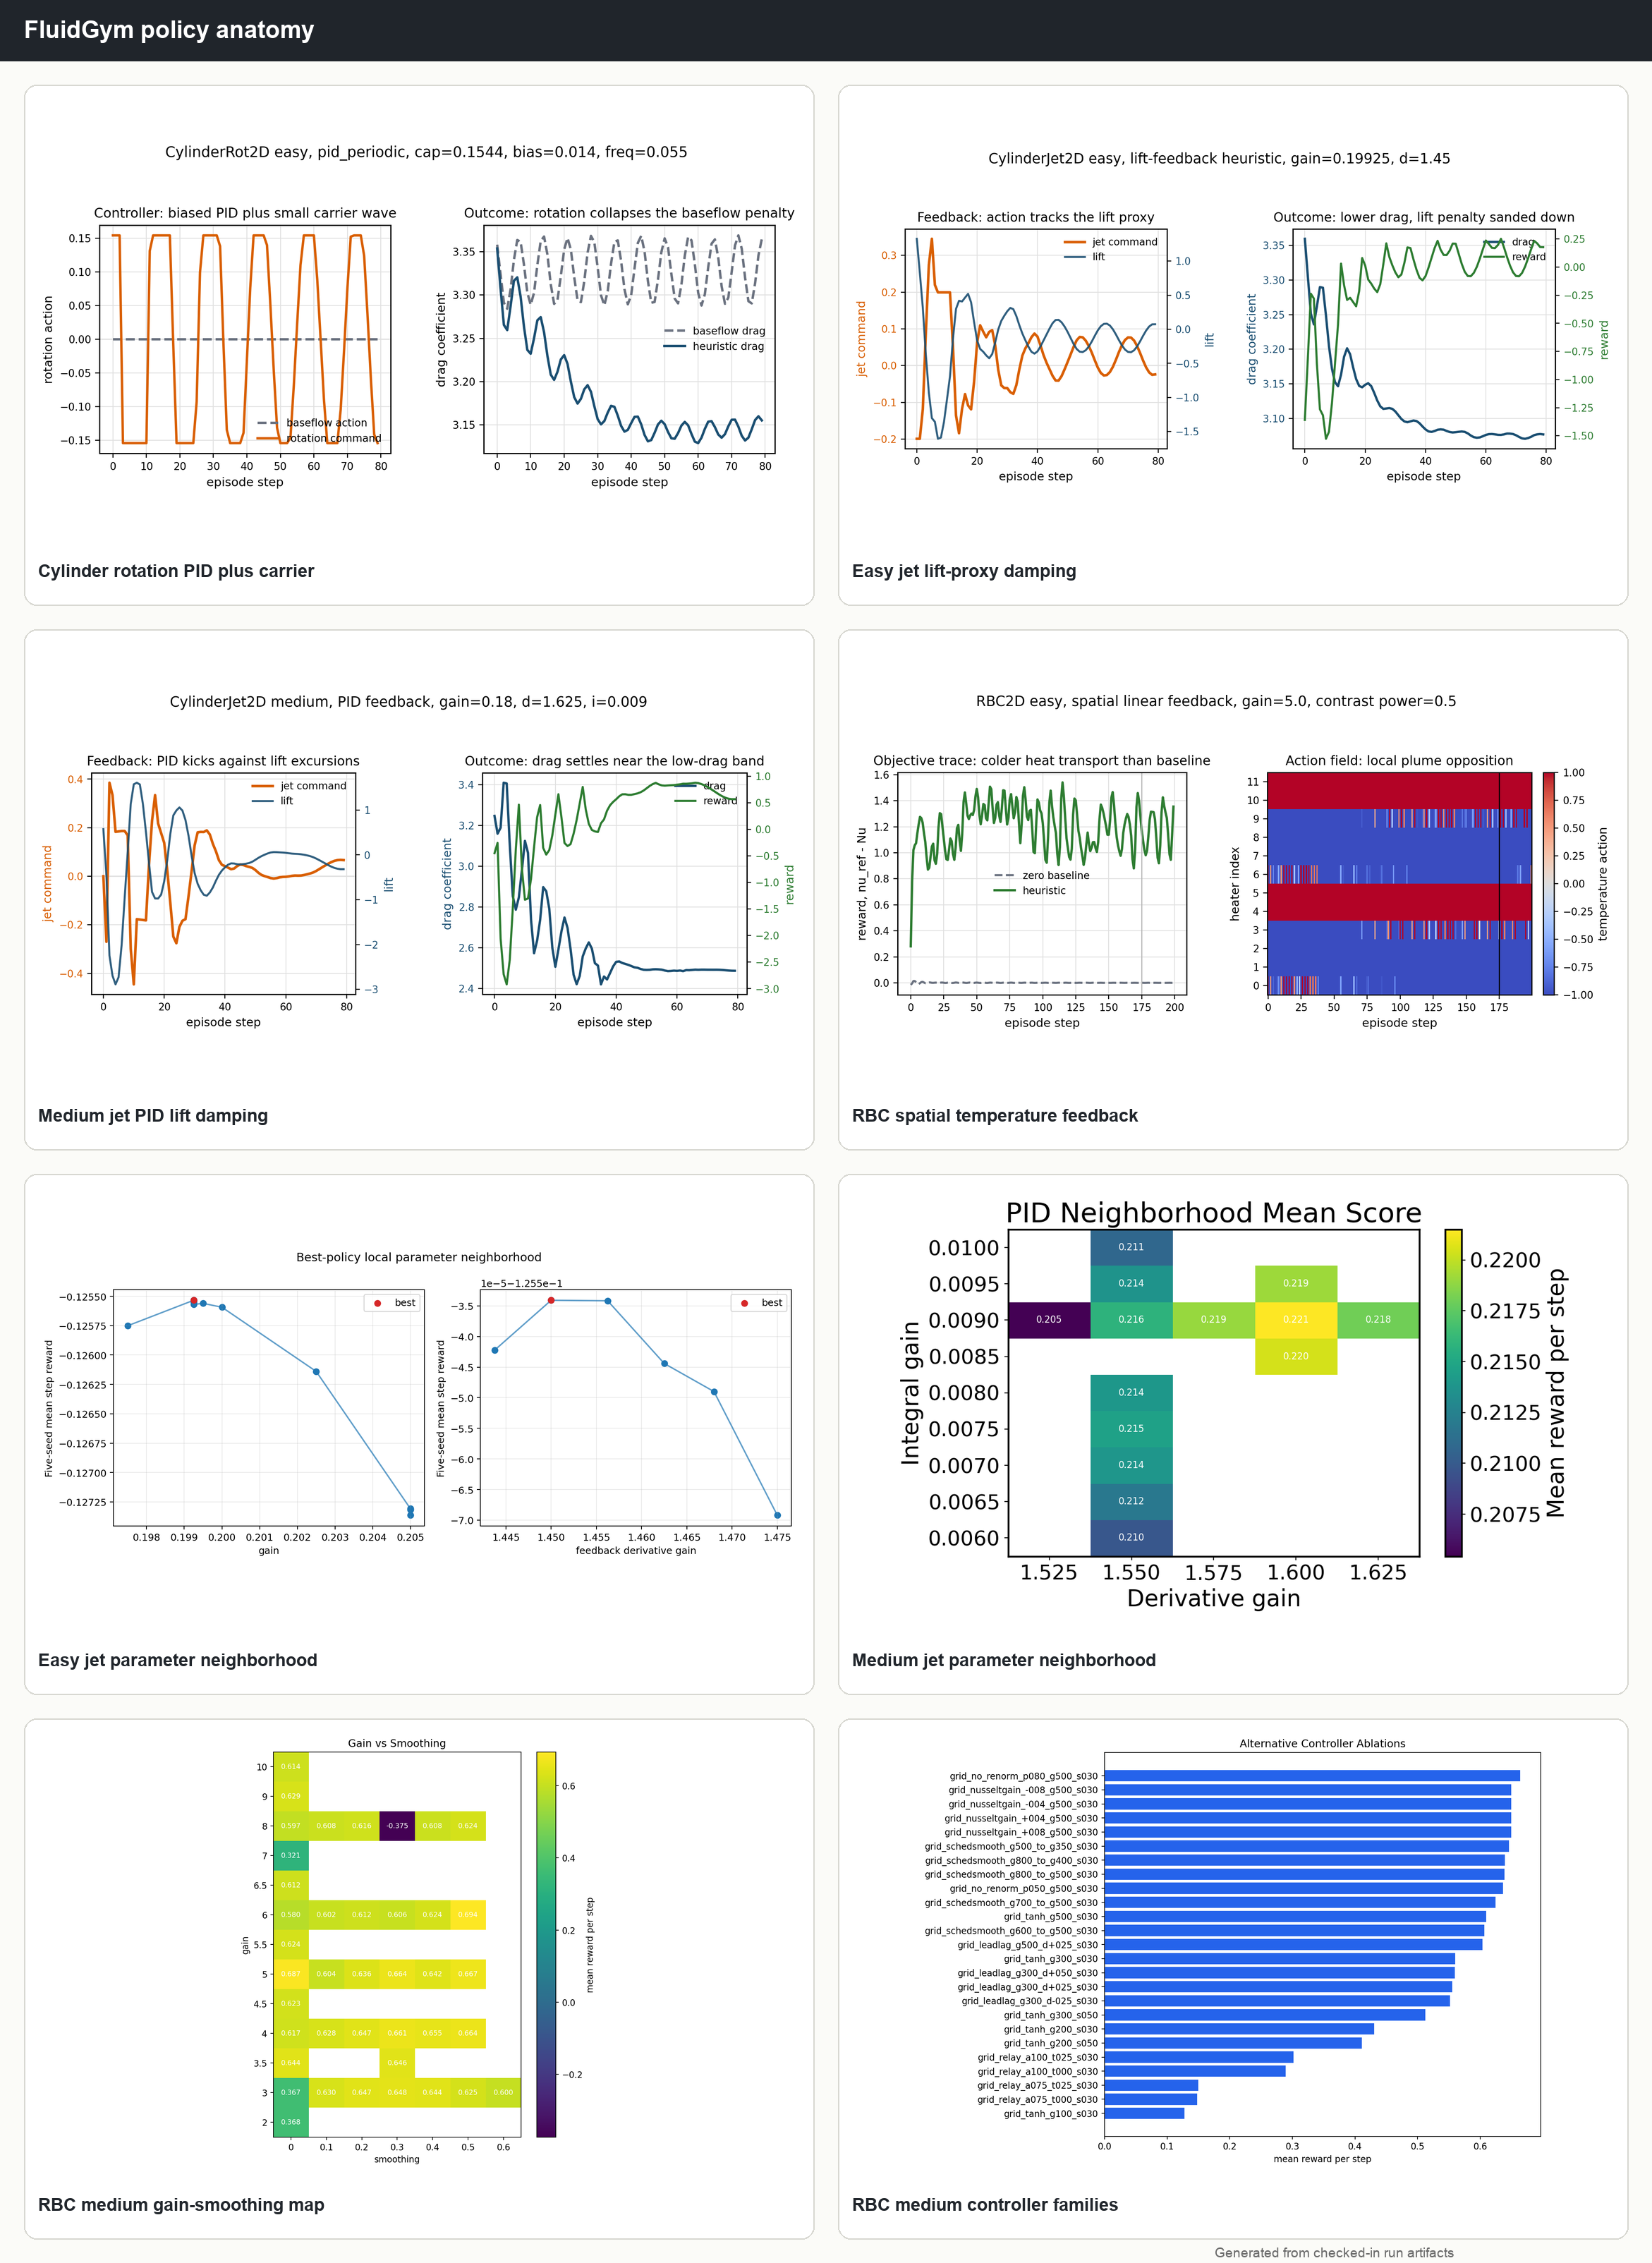
\includegraphics[width=\linewidth,height=0.82\textheight,keepaspectratio]{figures/fluidgym_strategy_gallery.png}
\caption{FluidGym policy anatomy and search diagnostics. The useful pattern is painfully concrete: small laws, clipped actions, local signals, and enough seed checking to catch the flashy failures.}
\end{figure}

\subsection{Cylinder Controls}

CylinderRot2D-easy is a wall-rotation controller with a capped PID-like law. The final selected config is:
\[
a_t = \operatorname{clip}\left(b - k_p L_t - k_d (L_t-L_{t-1}) + c\sin(2\pi f t), -A, A\right),
\]
with \(A=0.1544\), \(b=0.014\), \(k_p=-1.0\), \(k_d=-0.60\), \(c=0.005\), and \(f=0.055\). The replay cuts mean drag from \score{3.3279} to \score{3.1821}. The reward remains uglier than the drag story because the objective penalizes more than steady drag alone.

CylinderJet2D-easy uses the public observation vector to estimate lift through a 302-weight linear proxy. It sends:
\[
a_t=\operatorname{clip}\left[-0.19925\left(s_t + 1.45(s_t-s_{t-1})\right), -1, 1\right],
\]
where \(s_t\) is the clipped lift proxy. This is a good example of a heuristic that looks too simple until the proxy is counted. The fitted sensor map is doing real work.

CylinderJet2D-medium keeps the same shape but switches to public lift PID:
\[
a_t=\operatorname{clip}\left[-0.18\left(s_t + d(s_t-s_{t-1}) + 0.009 I_t\right), -1, 1\right],
\]
with \(d=1.60\) for the selected expected-score controller and \(d=1.625\) for the peak variant. The low-tail seed risk is real: the 15-seed mean is \score{0.2138}, while the best single trial is \score{0.2433}.

\subsection{RBC Controls}

RBC2D-easy is the cleanest engineered law in the FluidGym set. It takes the temperature channel, averages it under each of 12 heaters, removes the spatial mean, applies a signed square-root contrast transform, normalizes, mean-free projects the action, and clips to the action bounds:
\[
u_h = \operatorname{clip}\left[-5.0 \cdot
\frac{\operatorname{sgn}(z_h)|z_h|^{0.5}-\overline{\operatorname{sgn}(z)|z|^{0.5}}}{\sigma+10^{-8}}, -1, 1\right].
\]
The held-out result, \score{1.1093}, is the strongest FluidGym reward result in the bundle.

RBC2D-medium is the same law with smoothing \(\alpha=0.3\). It is promising and cheap, but the report should keep the caveat bolted to the row: final held-out validation was skipped after wrap-up. The grouped score of \score{0.6292} still beats most reported paper baselines except SAC.

\subsection{TCF Control}

TCFSmall3D-both-easy is the most persuasive case against assuming the learned policy is automatically better. The selected local law uses \(\alpha=0.263671875\), \(\beta_u=0.2109375\), one spatial smoothing pass, per-wall centering and normalization, same-sign top-wall actuation, clip \(0.30\), and mean-free projection. The best reward \score{0.3068} clears the MA-PPO reference \score{0.207}. The one-episode drag-reduction diagnostic reports \score{30.26\%} mean reduction and \score{41.93\%} final reduction.

\section{Beacon Results}

\begin{table}[H]
\centering
\small
\begin{tabularx}{\linewidth}{L{0.15\linewidth}L{0.22\linewidth}L{0.18\linewidth}Y}
\toprule
Beacon case & Policy & Replay result & Mechanism \\
\midrule
Lorenz & \code{lorenz\_threshold} & Return \score{477.0}; mean reward \score{0.954}; 500 steps. & Threshold state machine over \(x\) and \(dx/dt\); chooses action 0 or 2 to keep \(x<0\). \\
Rayleigh & \code{modal\_pd} & Best score \score{-113.3135}; mean Nusselt \score{1.1331}; target \score{-100} not reached. & Two active modes, normalized modal PD, zero-mean bottom temperature action, \(k_p=11.0807\), \(k_d=0.2457\), cap 0.6. \\
Mixing & Best valid wall-action policy & Best full-episode valid score \score{-7.4252}; target \score{-5} not reached. Invalid state-homogenizer boundary probe scores \score{-1.2969}. & Valid plateau is adaptive/cyclic wall shears. The stronger boundary probe applies \(\mathrm{env.C}[:, :] = \mathrm{mean}(\mathrm{env.C})\) after each step, so it directly edits simulator state. \\
Burgers & \code{burgers\_delay} & Return \score{-2.9603}; mean reward \score{-0.0148}; 200 steps. & Delayed feedback with gradient gain, smoothing, and a deadband. \\
Sloshing & \code{sloshing\_modal} & Return \score{-0.4414}; mean reward \score{-0.0368}; 12 steps. & Modal law with phase lead, smoothing 0.95, deadband, and second-mode gain. \\
Vortex & Piecewise-linear phase drift & Return \score{62.4213}; mean reward \score{0.0780}; target \score{100} not reached. & Near-maximum forcing amplitude, with the phase action linearly interpolated through 18 slowly drifting knots in \([-0.6231,-0.2568]\). \\
\bottomrule
\end{tabularx}
\caption{Beacon results for the non-Shkadov cases. Rayleigh, Mixing, and Vortex use the latest saved target-search artifacts where available; Lorenz, Burgers, and Sloshing remain the checked-in replay summaries.}
\end{table}

\begin{table}[H]
\centering
\small
\begin{tabularx}{\linewidth}{L{0.25\linewidth}r r r r Y}
\toprule
Shkadov case & Jets & Seeds & Hit rate & Mean score & Basis \\
\midrule
Older 5-actuator readable feedforward & 5 & 50 & \score{1/50} & \score{-3.4944} & Beat seed 0 at \score{-0.4711}, then failed seed sweep; useful as a falsified open-loop result. \\
Stable delayed shape feedback & 5 & 50 & \score{50/50} & \score{-0.3538} & Public observation only; worst seed \score{-0.4566}, best seed \score{-0.2480}. \\
Stable delayed shape feedback, wider sweep & 5 & 138 & \score{138/138} & \score{-0.3443} & Same controller; worst seed \score{-0.4632}, best seed \score{-0.2412}. No misses saved through seed 137. \\
Stable delayed shape feedback adapted to 10 jets & 10 & 50 & \score{50/50} & \score{-0.3967} & Same feature spine with delay 8, gain 0.28, smoothing 0.90, taper \(1.03^j\). Worst seed \score{-0.4904}. \\
\bottomrule
\end{tabularx}
\caption{Latest Shkadov results. The target is score \(>-0.5\); the stable feedback law clears it across the saved random-reset sweeps.}
\end{table}

\begin{figure}[H]
\centering
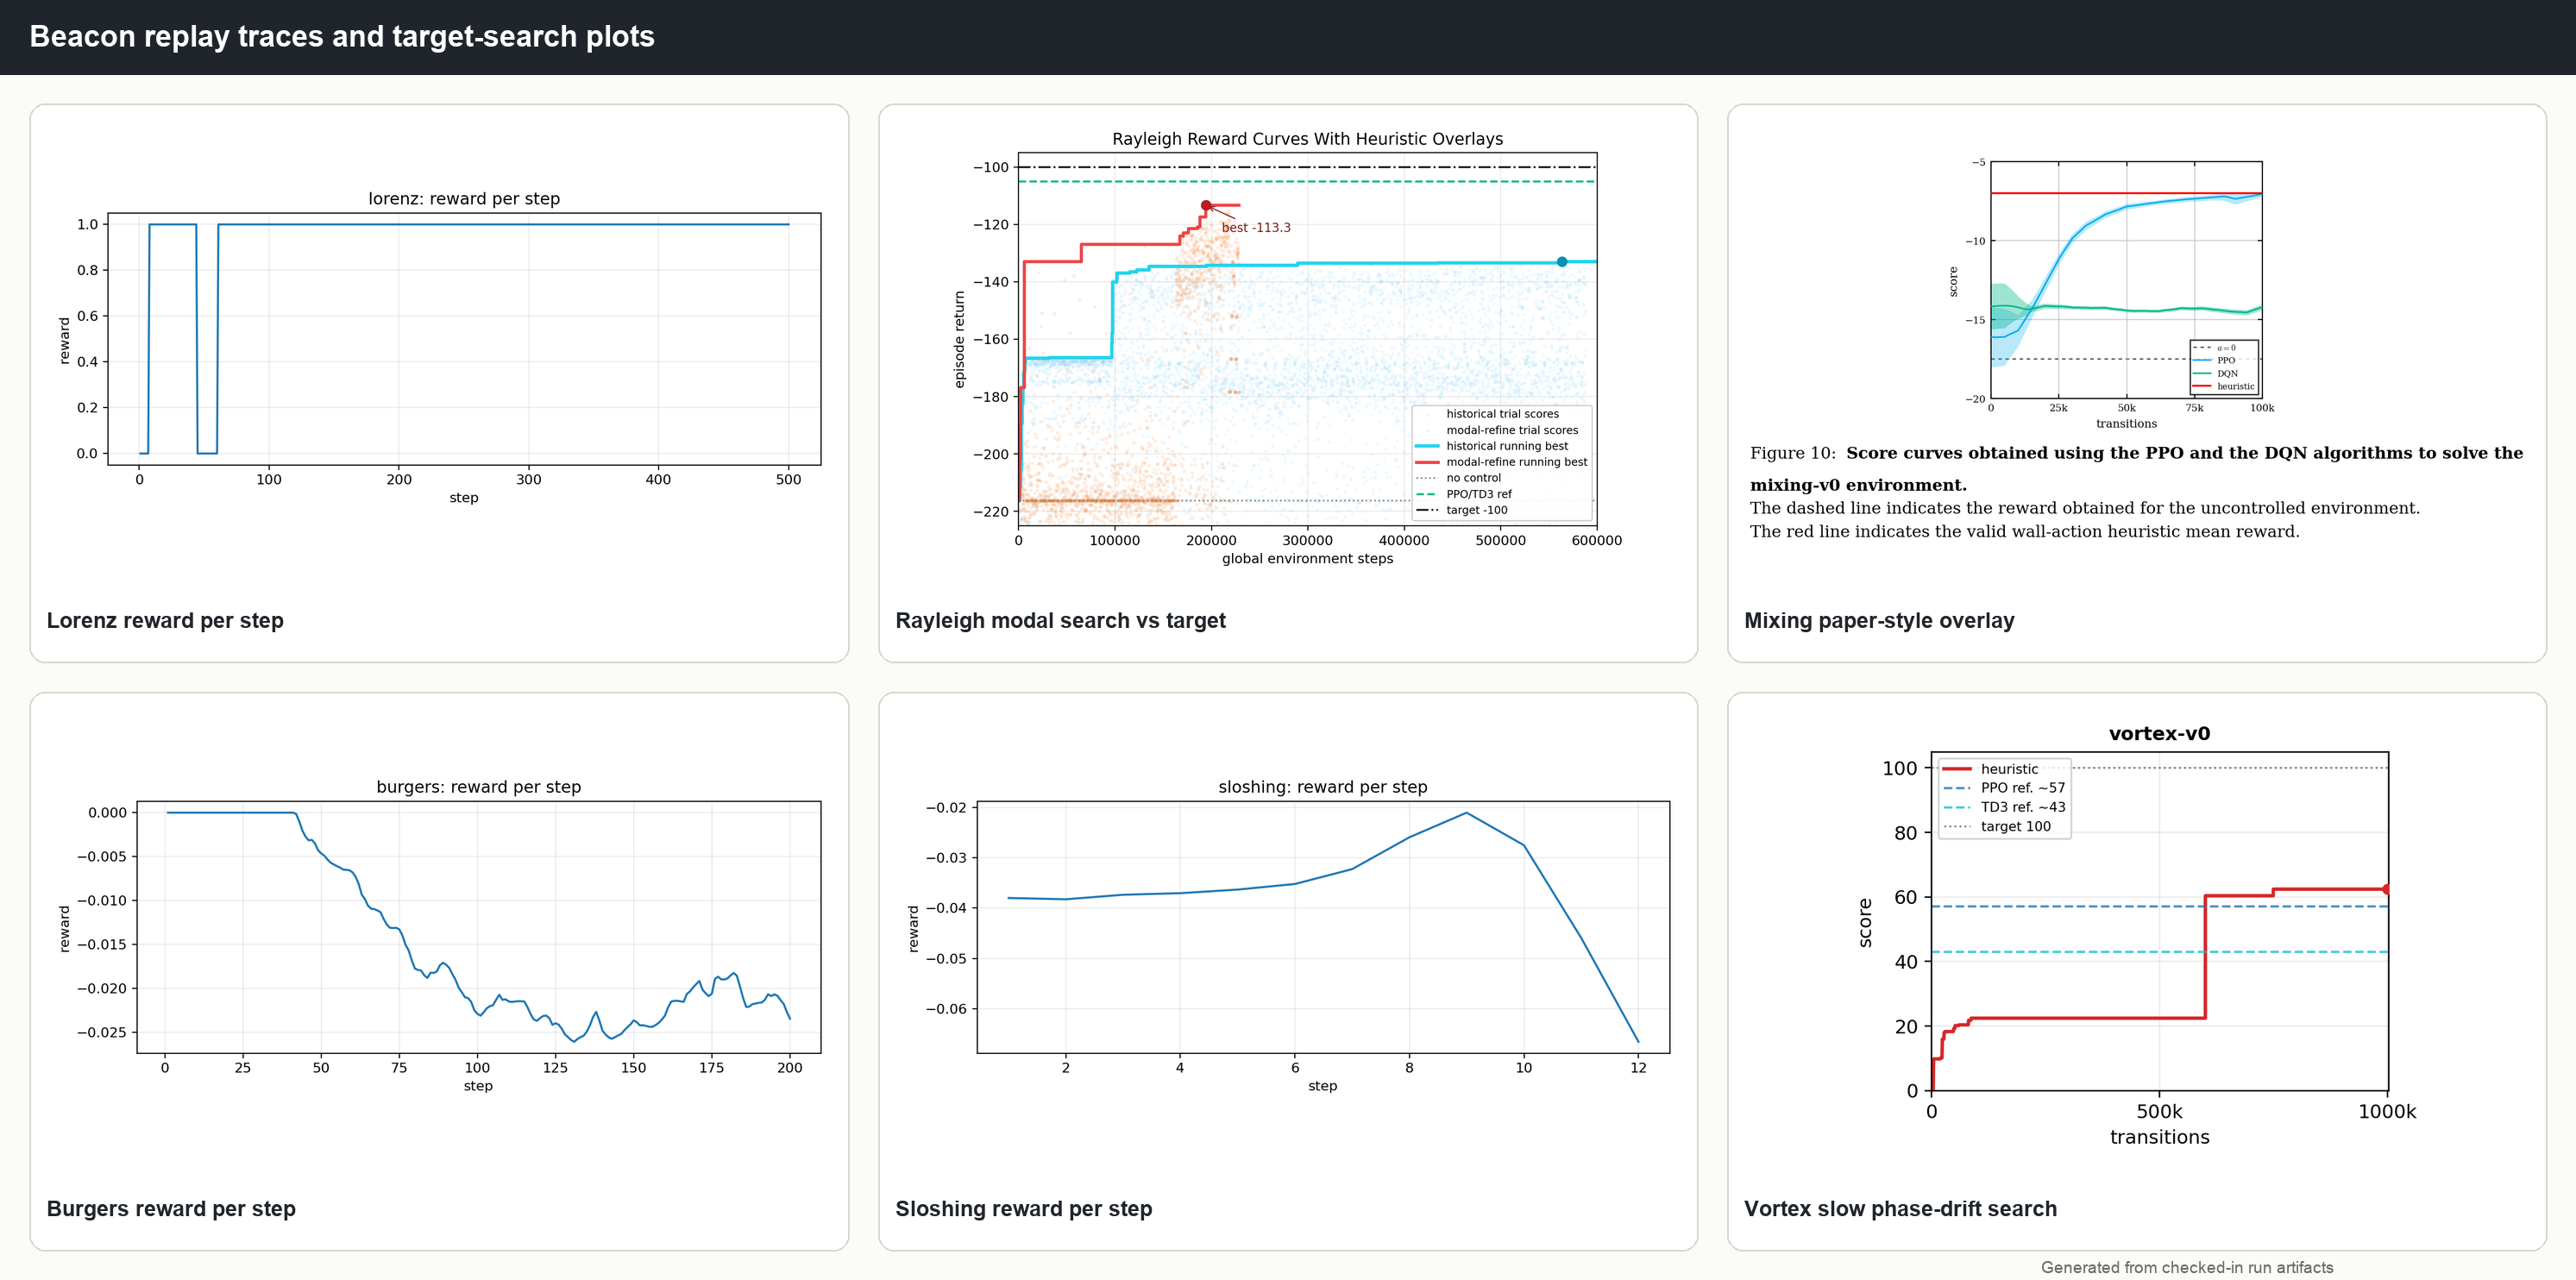
\includegraphics[width=\linewidth]{figures/beacon_replay_gallery.png}
\caption{Beacon reward traces and target-search plots. The gallery now separates old replay traces from the latest May 15 target runs where those exist.}
\end{figure}

\begin{figure}[H]
\centering
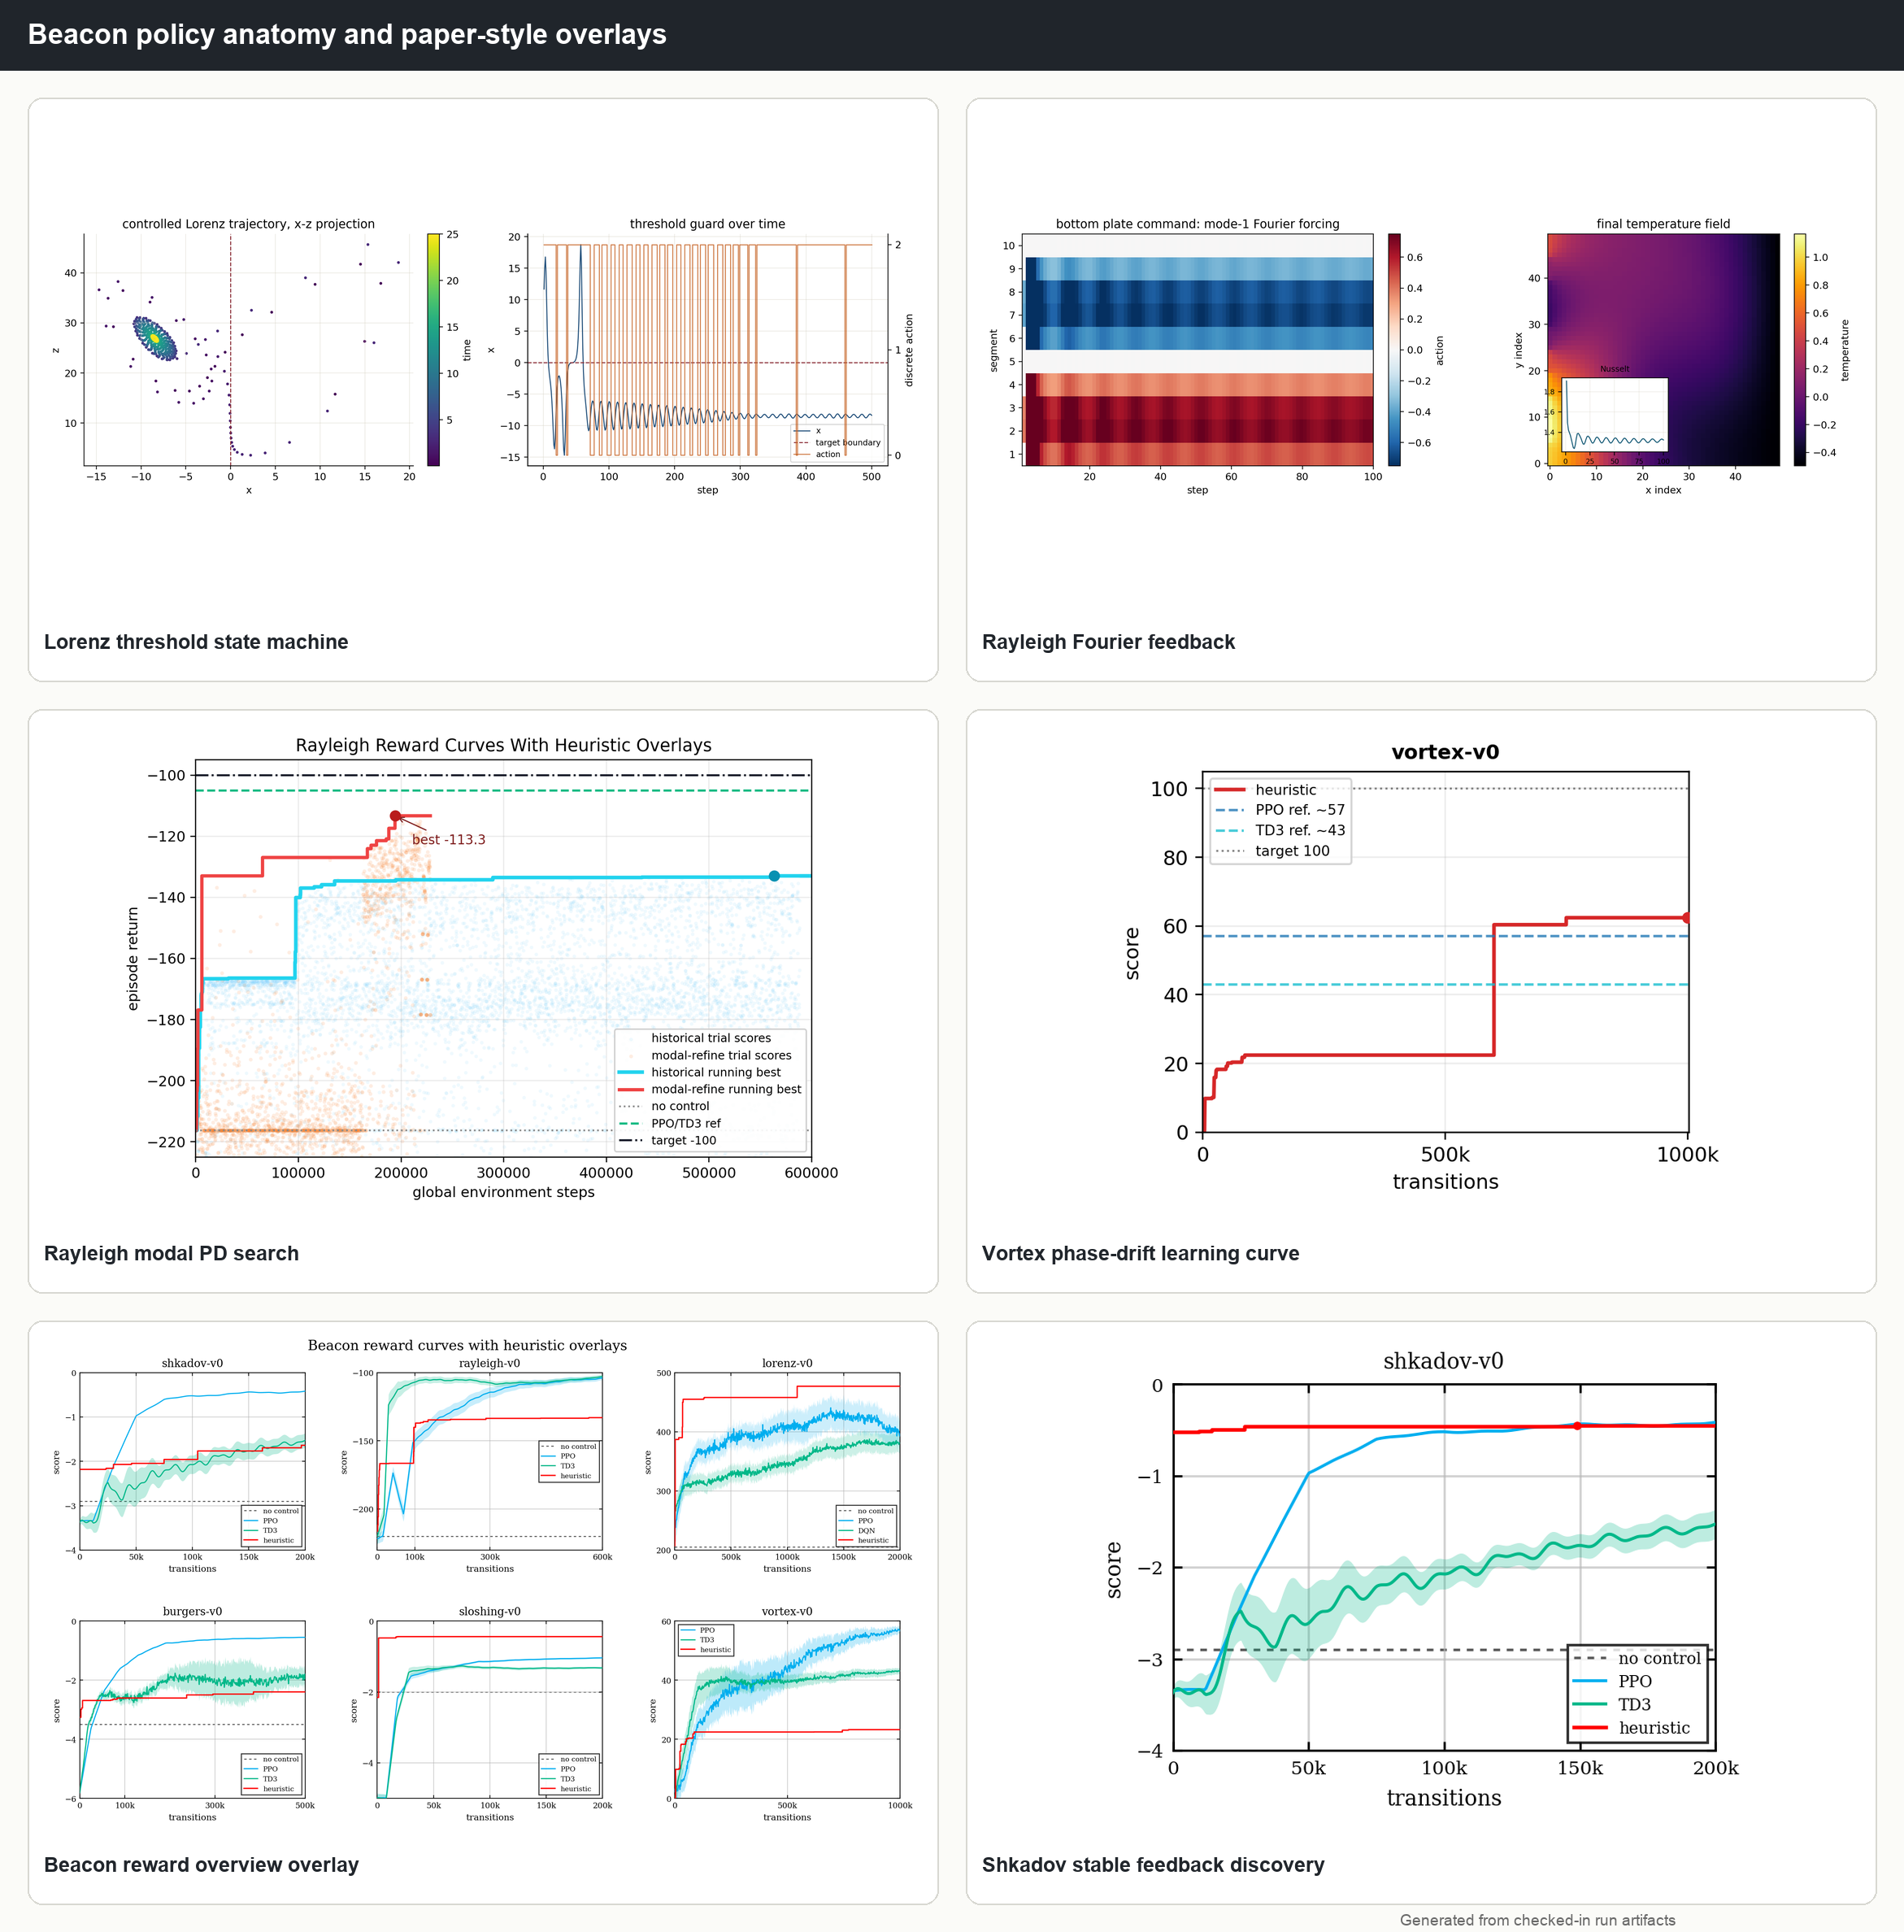
\includegraphics[width=\linewidth]{figures/beacon_strategy_gallery.png}
\caption{Beacon policy anatomy and paper-style overlays. Lorenz is a threshold automaton, Rayleigh is modal PD, Vortex is slow phase drift, and Shkadov is delayed local shape feedback.}
\end{figure}

\begin{figure}[H]
\centering
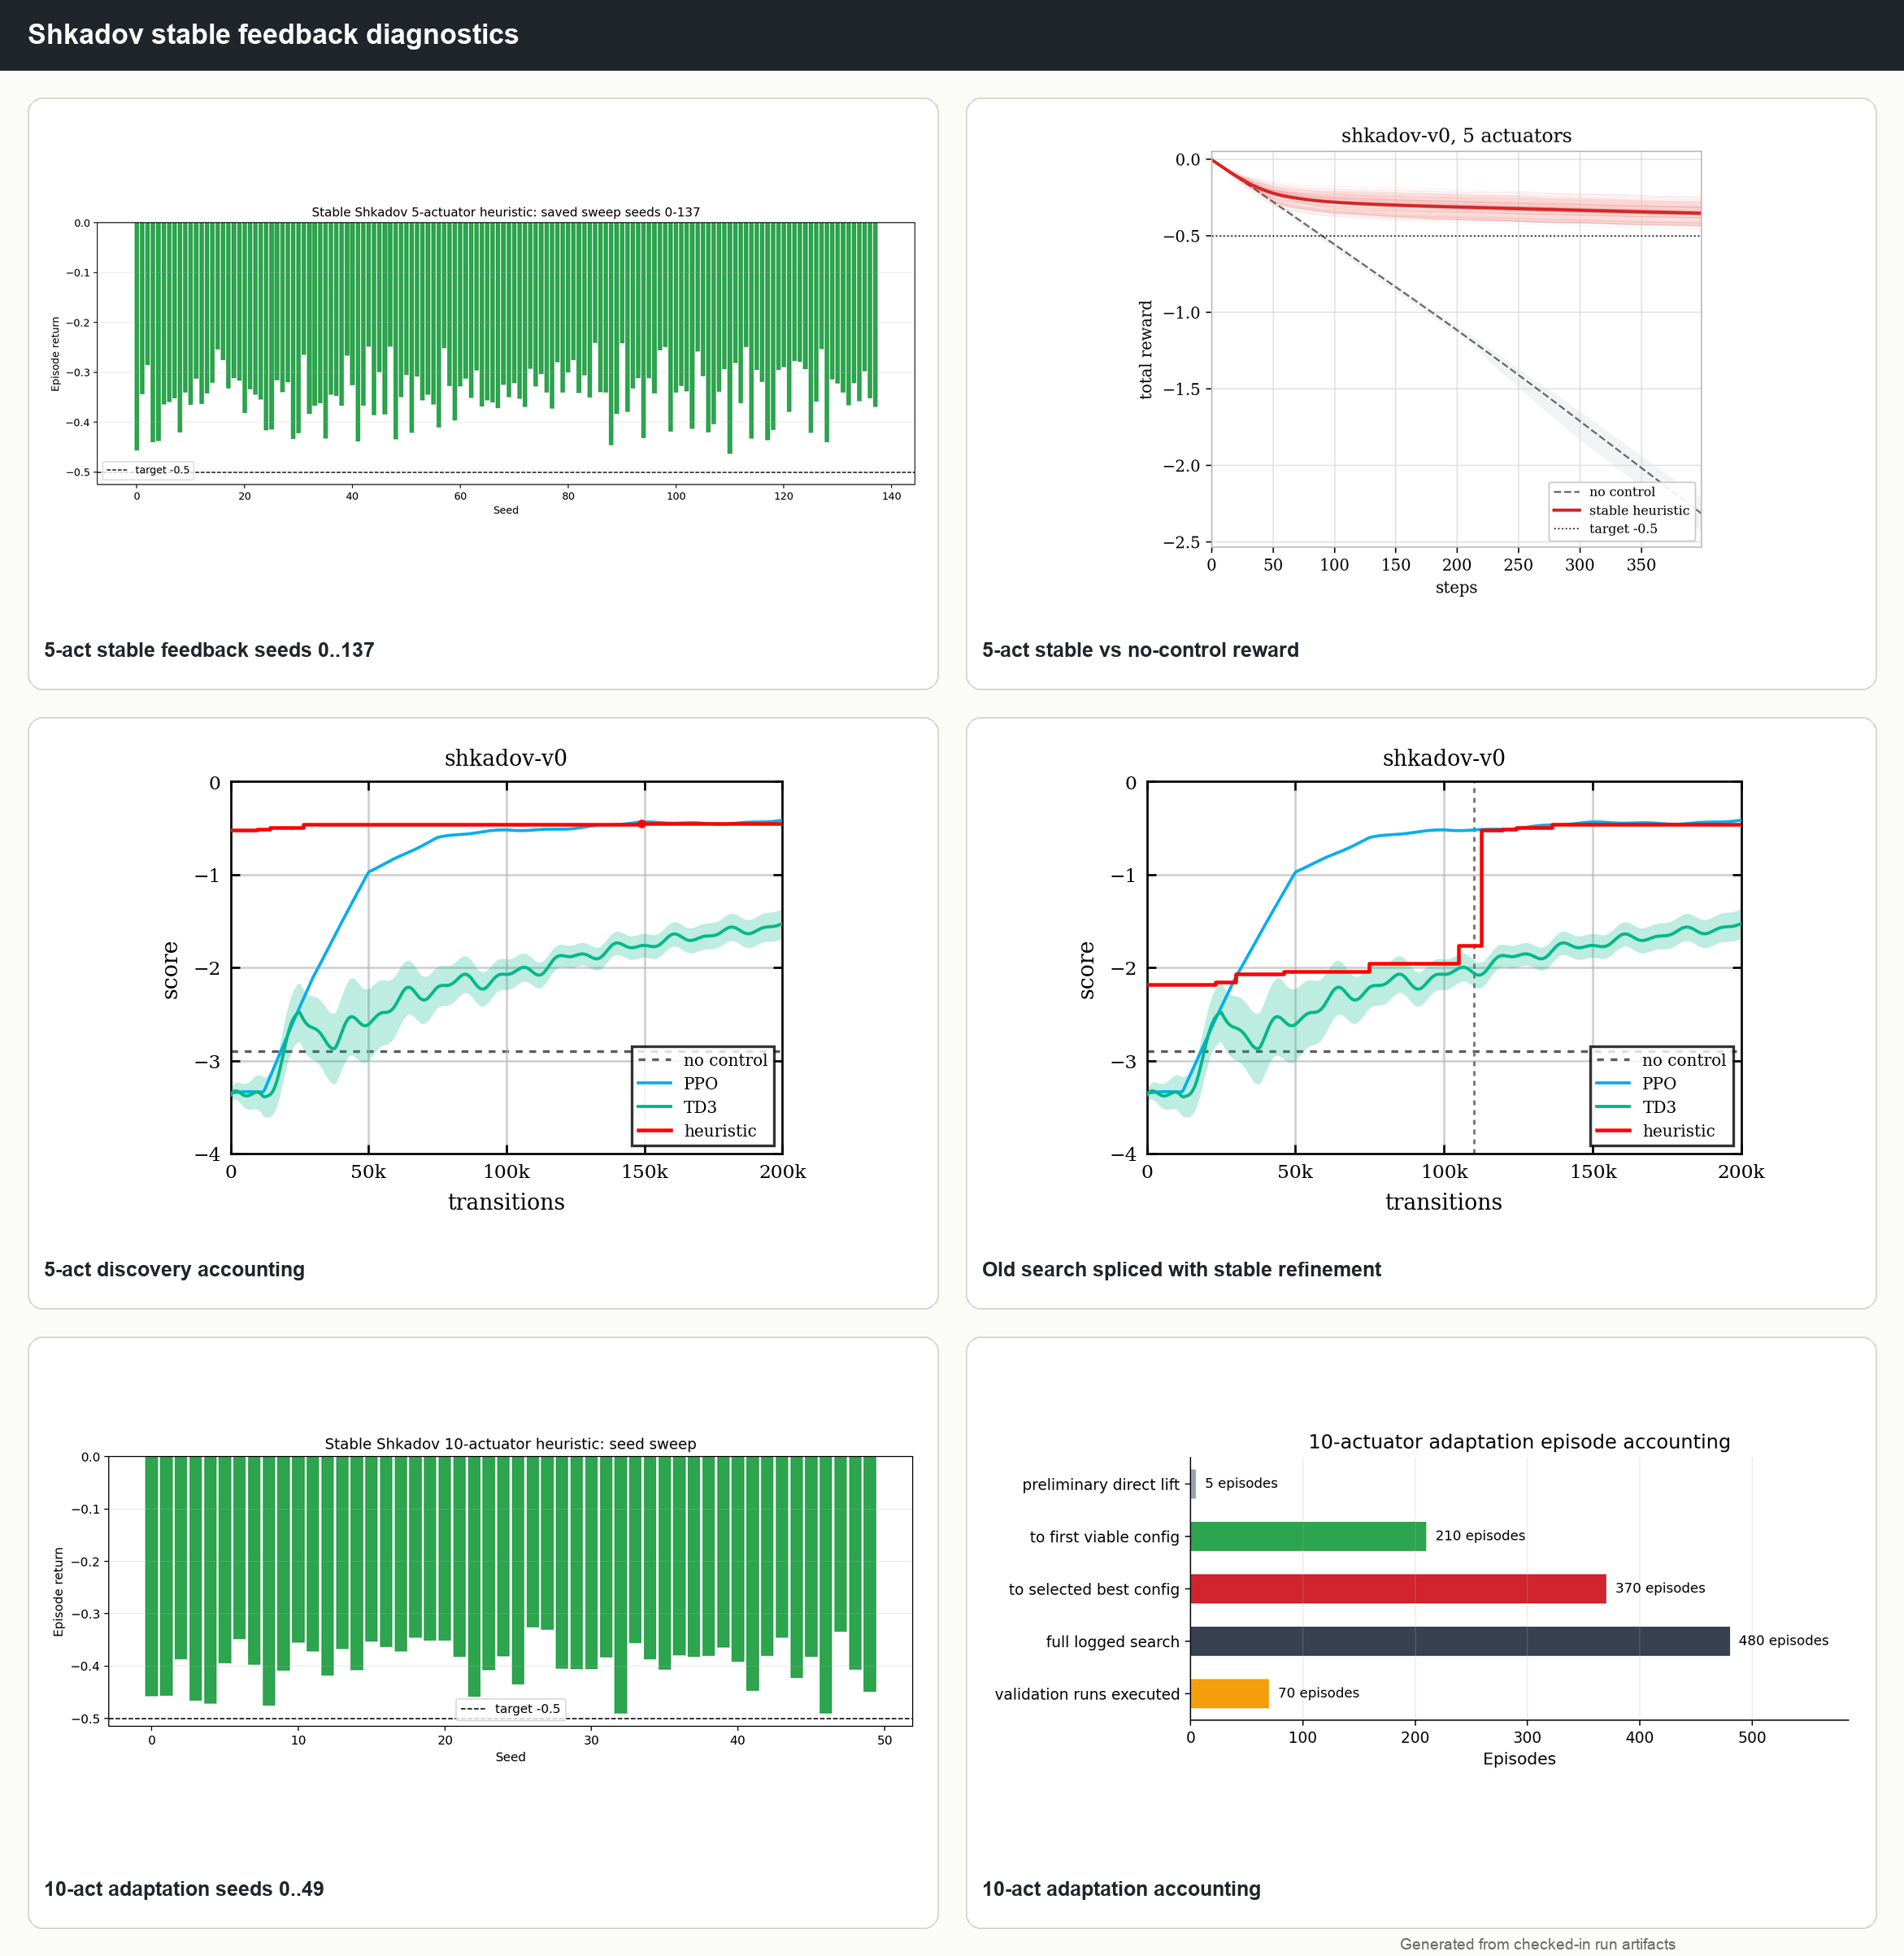
\includegraphics[width=\linewidth]{figures/shkadov_gallery.png}
\caption{Shkadov diagnostics. The old transfer bundle is now mainly a negative control; the stable delayed-feedback law is the current result.}
\end{figure}

\section{Policy Families}

The explicit formulas in Sections 3 and 4 are physical recipes rather than lucky recipes. Each controller is a compressed answer to what the flow makes hard. The physics sets the obstacle, the obstacle shapes the search, and the final control law records the compromise that survived.

\begin{table}[H]
\centering
\scriptsize
\begin{tabularx}{\linewidth}{L{0.17\linewidth}Y Y Y}
\toprule
Case or family & Physical obstruction & Why the search is hard & Shape of the final control \\
\midrule
Rayleigh & Buoyant convection is a coupled roll problem. Bottom heating creates plume growth, vertical transport, and recirculation; reducing Nusselt means cutting heat transport without simply dumping a biased wall temperature into the domain. & The controller has two passes to clear. First it must knock down the near-wall plume or roll phase. Then it must stop the remaining circulation from rebuilding the same convective cell one turnover later. Constant forcing does nothing in the saved sweep, and many local laws either leave the roll intact or inject the wrong phase. & Zero-mean modal-PD bottom forcing over modes 1 and 2. The latest saved controller is vertical-velocity dominated (\(v_w=-0.7320\)), normalized, smoothed at 0.5, and capped at 0.6. That shape reads like roll-phase and momentum damping rather than global thermal bias. \\
RBC & The useful signal is local thermal contrast under each heater, while the bad move is bulk heating or cooling that changes the mean but leaves the convective structure alive. & A scalar control can look energetic and still miss the geometry. The search has to preserve actuator locality, avoid mean drift, and avoid overreacting to one heater's noisy temperature sample. & Mean-free spatial temperature feedback. The square-root contrast transform gives large plumes enough authority without letting one segment pin the action box forever. \\
TCF & Drag reduction depends on shaping near-wall streaks on both walls rather than pushing the whole wall in one direction. & Wrong wall signs and scalar wall-stress feedback fail because they erase the spatial information the actuator grid exposes. The search has to keep translation structure while matching top and bottom signs. & Per-wall centered, normalized, lightly smoothed local feedback with a mean-free projection. The final law is spatially organized because the drag-producing structure is spatially organized. \\
Cylinder jets & The control target is vortex shedding. The public signal is an indirect lift or lift-proxy trace, so timing matters more than raw actuation amplitude. & The delay between sensing, actuation, and wake response means a pure proportional law chases the past. Seed tails appear when the phase relation slips. & PID-like lift damping with derivative memory, clipping, and in the easy case a learned linear lift proxy from the public sensor vector. \\
Shkadov & The film-height error is downstream of the jets. With multiple jets, the actuator can shape the surface before the reward station sees it. & Reactive feedback is late because the reward is spatially downstream. The search only becomes stable once it stops chasing the immediate height sample and builds a delayed local shape proxy. & Delayed local shape feedback. The stable 5-jet law uses actuator-local mean, slope, curvature, and last-point deviation, delays the signal by 11 steps, tapers it downstream, deadbands it, and smooths the action at 0.84. \\
\bottomrule
\end{tabularx}
\caption{Physics-to-control bridge. This is the missing connective tissue between the explicit heuristics and the policy-family taxonomy.}
\end{table}

Rayleigh-v0 is the best warning against treating the formula as a mere search artifact. In the latest modal-PD replay, Nusselt drops from \score{1.8259} at step 0 to \score{1.3103} by step 12 and reaches \score{1.0476} at step 16. Late in the episode it still oscillates between roughly \score{1.00} and \score{1.31}. That pattern is the two-pass problem in numbers: the first pass suppresses the initial convective transport, the second pass has to keep the roll from reconstituting after the flow has had time to circulate.

That also explains the final control's asymmetry. The action is zero-mean, uses modes 1 and 2, and puts high authority into a clipped spatial pattern across the bottom plate. The useful authority goes into phase and velocity damping against the dominant circulation rather than into a global wall-temperature offset.

\textbf{Scalar feedback with memory.} CylinderJet, CylinderRot, Burgers, Sloshing, and Vortex all live in this family. The formula changes, but the spine is the same: measure one scalar or phase-like signal, add derivative or phase memory, smooth it, deadband it, clip it. The best versions are boring in the productive sense. They make the actuator move only when the signal earns it.

\textbf{Spatial mean-free laws.} RBC and TCF are the serious spatial controllers. They strip off the global mean, act on local contrast, and respect the actuator geometry. The mean-free projection matters because these environments punish global heating or bulk wall forcing that looks energetic but fails the physics.

\textbf{Delayed local shape feedback.} Shkadov 5 jets is now the main Beacon seed-sweep win. For each actuator-local upstream \(q\) window, the controller computes mean, slope, curvature, and last-point deviation, delays the signal by 11 steps, tapers it downstream, adds a small bias, clips, deadbands, and smooths:
\[
\mathrm{signal}_j =
\mathrm{mean}_j
-0.5847514\,\mathrm{slope}_j
+0.9217264\,\mathrm{curve}_j
-0.2278599\,\mathrm{last}_j,
\]
\[
a_{j,t}=0.16\,\operatorname{deadband}_{0.05}
\left(\operatorname{clip}\left[-0.3475133\,\mathrm{signal}_{j,t-11}\,0.95^j+0.0263648,-1,1\right]\right)
+0.84\,a_{j,t-1}.
\]
The 10-actuator adaptation keeps the same feature spine but shortens the delay to 8, lowers gain to 0.28, increases smoothing to 0.90, and changes the taper to \(1.03^j\).

\textbf{Threshold automata.} Lorenz is the purest version: use \(x\) and \(dx/dt\), hold for one step, switch between two actions. It scores \score{477/500}. That number is so high because the benchmark reward is brutally aligned with the threshold condition \(x<0\).

\textbf{Proxy-based control.} CylinderJet2D-easy is the warning label. Calling it a simple heuristic undersells the 302-weight lift proxy. The control law is small; the public-observation compression is carrying much of the intelligence.

\section{Comparison to Learned Baselines}

\begin{figure}[H]
\centering
\begin{subfigure}{0.49\linewidth}
  \includegraphics[width=\linewidth]{../paper/plots/env_suite/fluidgym_beacon_policy_comparison.png}
  \caption{Policy comparison overview.}
\end{subfigure}
\hfill
\begin{subfigure}{0.49\linewidth}
  \includegraphics[width=\linewidth]{../paper/plots/env_suite/fluidgym_beacon_sample_efficiency.png}
  \caption{Sample-efficiency overview.}
\end{subfigure}
\caption{Checked-in environment-suite overview plots. These give the broad context for the individual case results above.}
\end{figure}

The clean wins are RBC2D-easy and TCFSmall3D-both-easy. RBC2D-easy's held-out reward beats the paper table's MA-PPO reward. TCFSmall3D-both-easy beats both MA-PPO and MA-SAC references on reward and has a direct drag-reduction plot.

The cylinder jet story is respectable but less dominant. Easy gets close to SAC drag improvement. Medium reaches D-MPC-level reward on the peak score and slightly below that on the 15-seed expected controller, but SAC remains ahead.

RBC2D-medium is a transfer result. The grouped score is good enough to matter, but the missing final held-out rerun blocks a stronger claim. The right wording is: promising transfer, ahead of several paper baselines, below SAC, pending held-out replay.

Beacon comparisons should stay case-specific. Lorenz is excellent because the reward target is simple. Shkadov is now a genuine stable heuristic result, with 138 saved random-reset seeds clearing the \(-0.5\) target. Vortex has a solid bounded-action improvement but plateaus near \score{62.4}, below the \score{100} target. Rayleigh is close to the paper-visual PPO/TD3 reference but still below the \(-100\) target. Mixing remains unsolved under the valid wall-action-only constraint; the impressive \(-1.2969\) boundary probe edits simulator state and belongs in the negative-results bin.

\section{Negative Results}

The failures are as useful as the wins. Across FluidGym, the discarded branches include row pruning, alternate sensor grouping, pure relay control, tanh saturation, one-heater rolls, post-clip zero-mean projection, public-Nusselt adaptive gain, open-loop waves for the cylinder tasks, flipped TCF top-wall signs, scalar wall-stress feedback, event gating, low-pass delay, and \(u v\) cross terms.

That failure list tells the real story. The best policies survive because they match actuator geometry and benchmark observables. The failed ones usually inject energy, erase spatial structure, or chase a delayed scalar after the flow has already moved on.

Beacon adds sharper failure labels. Mixing wall actions have not beaten \(-5\); the best valid full-episode score saved here is \score{-7.4252}. Vortex phase-lock feedback was beaten by open-loop slow phase drift, but the search still stalled far below \score{100}. Rayleigh modal control is close but not target-clearing. Old Shkadov feedforward hit one seed and collapsed over 50; stable delayed feedback fixed that specific brittleness.

\section{Final Assessment}

The report's strongest claim is narrow and defensible: \textbf{structured heuristics can beat or approach expensive learned baselines on selected FluidGym and Beacon control tasks when the observation geometry exposes the right signal.}

The weaker claim would be that heuristic search has solved the suite. It hasn't. Airfoil cases aren't represented in this heuristic bundle. RBC2D-medium still needs held-out replay. Beacon evidence is split: Shkadov is seed-checked, Vortex is improved but target-short, Rayleigh is close but target-short, and Mixing remains unsolved under the valid actuator-only rule.

The useful research direction is clear: treat learned policies as a source of geometry and timing hints, then compress those hints into tiny laws with explicit seed checks. The winning artifacts here are readable, replayable, and falsifiable. That last word matters. A black-box policy can win a plot; a 12-line control law can explain why it won.

\appendix
\section{Audit Trail}

\begin{longtable}{L{0.28\linewidth}L{0.66\linewidth}}
\toprule
Result & Local source \\
\midrule
CylinderRot2D-easy validation & \path{cylinder_rot_2d_easy_24h/final_validation_summary.json} and \path{cylinder_rot_2d_easy_24h/final_action_drag_timeseries.csv}. \\
CylinderJet2D-easy validation & \path{cylinder_jet_2d_easy/top_policy_summary.csv}, \path{cylinder_jet_2d_easy/best_policy_manifest.json}, and \path{cylinder_jet_2d_easy/easy_experiment_wrapup.md}. \\
CylinderJet2D-medium validation & \path{cylinder_jet_2d_medium_24h_improvement/final_best_heuristic_run_summary.json} and \path{cylinder_jet_2d_medium_24h_improvement/best_heuristic_medium_seed_scores.csv}. \\
RBC2D-easy validation & \path{rbc_2d_easy_24h_final/FINAL_WRAPUP.md}, \path{rbc_2d_easy_24h_final/final_run_stats.json}, and \path{rbc_2d_easy_24h_final/final_plots/best_heuristic_test_episode_metrics.json}. \\
RBC2D-medium transfer & \path{rbc_2d_medium_transfer_50k/transfer_report.md} and \path{rbc_2d_medium_transfer_50k/best_policy_manifest.json}. \\
TCFSmall3D-both-easy & \path{tcf_small_3d_both_easy_heuristic_package/run_artifacts/FINAL_REPORT.md}, \path{best_policy_manifest.json}, and \path{heuristic_one_episode_drag_reduction_summary.json}. \\
Beacon summaries & \path{beacon/lorenz/summary.json}, \path{beacon/rayleigh_target_minus_100/best_modal_nusselt/manifest.json}, \path{beacon/mixing_target_minus_5/README.md}, \path{beacon/burgers/summary.json}, \path{beacon/sloshing/summary.json}, \path{beacon/vortex_target_100_attempt/manifest.json}. \\
Shkadov summaries & \path{beacon/shkadov_stable_search/stable_feedback_seed_sweep_0_49_summary.json}, \path{beacon/shkadov_stable_search/stable_feedback_seed_sweep_0_137_summary.json}, \path{beacon/shkadov_stable_search/stable_feedback_total_reward_per_step_0_49_summary.json}, and \path{beacon/shkadov_stable_search/ten_actuator_adaptation/stable_feedback_10act_seed_sweep_0_49_summary.json}. \\
Strategy descriptions & \path{best_heuristic_strategy_notes/README.md} and \path{beacon/heuristic_strategy_descriptions/strategy_explanations.md}. \\
Comparison baselines & \path{paper/tables/Cylinder_results_table.tex}, \path{paper/tables/RBC_results_table.tex}, and \path{paper/tables/TCF_results_table.tex}. \\
\bottomrule
\end{longtable}

\section{Generated Contact Sheets}

The contact sheets were generated by:

\begin{verbatim}
python3 report/build_galleries.py
\end{verbatim}

The script reads existing plots and writes:
\begin{itemize}
\item \path{report/figures/fluidgym_replay_gallery.png}
\item \path{report/figures/fluidgym_strategy_gallery.png}
\item \path{report/figures/beacon_replay_gallery.png}
\item \path{report/figures/beacon_strategy_gallery.png}
\item \path{report/figures/shkadov_gallery.png}
\end{itemize}

\end{document}
